\documentclass[11pt]{standalone}
\usepackage{amssymb}
\usepackage{amsmath}

\usepackage[no-math]{fontspec}
\usepackage{unicode-math}
\setmainfont{Libertinus Sans}
\setsansfont{Libertinus Sans}
\setmathfont{Libertinus Math}

\usepackage{pgf,xcolor}
\usepackage{tikz}
\usetikzlibrary{arrows.meta, backgrounds}
\usepackage{pgfplots}
\pgfplotsset{compat=newest}
\usepackage{pifont}

\definecolor{my_darkgray}{HTML}{484949}
\definecolor{my_lightgray}{HTML}{F3F4F4}
\definecolor{my_darkblue}{HTML}{005A94}
\definecolor{my_lightblue}{HTML}{CCDEE9}
\definecolor{my_yellow}{HTML}{FFEC7F}
\definecolor{my_red}{HTML}{E60000}
\definecolor{my_orange}{HTML}{E87846}

\begin{document}
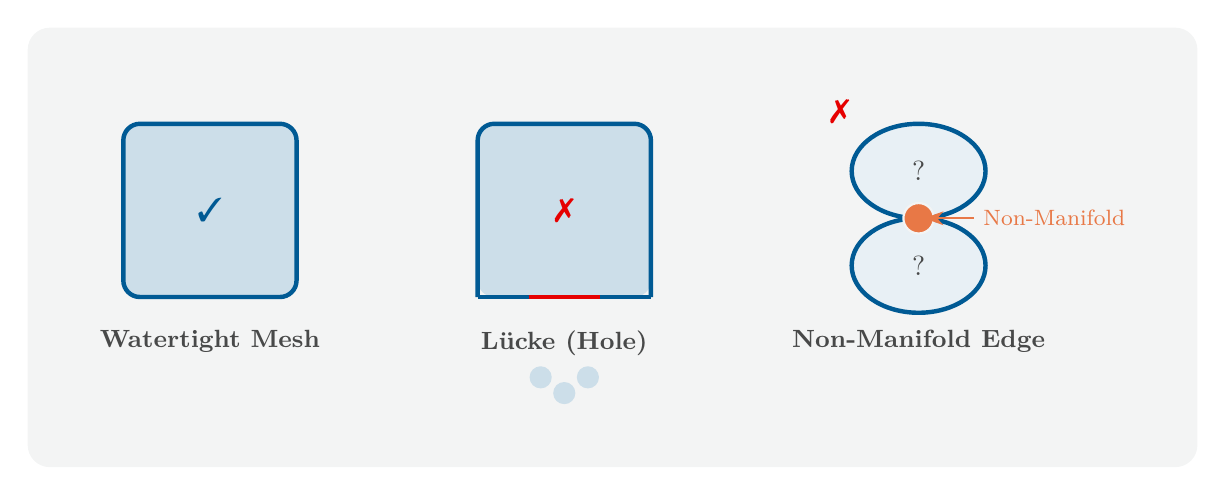
\begin{tikzpicture}[
    show background rectangle,
    background rectangle/.style={fill=my_lightgray, rounded corners=8pt},
    inner frame sep=0.8cm,
    annotation/.style={draw=my_darkgray, thick, -{Stealth[length=7pt, width=5pt]}}
]

% Alle drei Panels zeigen einen Mesh-Querschnitt (Ansicht von oben).
% Panels 1 und 2: geschlossenes Rechteck als Querschnitt der Mesh-Kontur.
% Panel 3: Zwei Ellipsen, die sich in einem Punkt berühren (Figur-8).
%
% Panel-Breite:  ca. 2.2 cm  (x: 0.4 bis 2.6)
% Panel-Höhe:    ca. 2.2 cm  (y: 0.4 bis 2.6)
% Panel-Abstand: 4.5 cm (xshift)

% ================================================================
% PANEL 1: Watertight Mesh (geschlossene Kontur)
% ================================================================

% Innenfüllung (Wasser)
\fill[my_lightblue, rounded corners=6pt] (0.4, 0.4) rectangle (2.6, 2.6);
% Kontur (geschlossen)
\draw[my_darkblue, ultra thick, rounded corners=6pt] (0.4, 0.4) rectangle (2.6, 2.6);

% Positivzeichen
\node[font=\large\bfseries, text=my_darkblue] at (1.5, 1.5) {\ding{51}};

% Panel-Titel
\node[font=\small\bfseries, text=my_darkgray, anchor=north] at (1.5, 0.1)
    {Watertight Mesh};

% ================================================================
% PANEL 2: Lücke (Hole)
% ================================================================
\begin{scope}[xshift=4.5cm]

% Innenfüllung (Wasser, auch bei Lücke zunächst gefüllt)
\fill[my_lightblue, rounded corners=6pt] (0.4, 0.4) rectangle (2.6, 2.6);

% Kontur mit Lücke am unteren Rand (Lücke: x = 1.05 bis 1.95)
% Linke Seite, oben, rechte Seite (mit rounded corners an den Ecken oben)
\draw[my_darkblue, ultra thick, rounded corners=6pt]
    (2.6, 0.4) -- (2.6, 2.6) -- (0.4, 2.6) -- (0.4, 0.4);
% Untere Kante rechts (bis zur Lücke)
\draw[my_darkblue, ultra thick] (2.6, 0.4) -- (1.95, 0.4);
% Untere Kante links (von der Lücke)
\draw[my_darkblue, ultra thick] (1.05, 0.4) -- (0.4, 0.4);

% Lücke hervorgehoben (my_red)
\draw[my_red, ultra thick] (1.05, 0.4) -- (1.95, 0.4);

% Wassertropfen unterhalb der Lücke
% (y-Positionen weit genug unter dem Panel-Titel, damit kein Overlap entsteht)
\foreach \xd/\yd in {1.2/-0.62, 1.5/-0.82, 1.8/-0.62} {
    \fill[my_lightblue] (\xd, \yd) circle (4pt);
}

% Negativzeichen
\node[font=\large\bfseries, text=my_red] at (1.5, 1.5) {\ding{55}};

% Panel-Titel
\node[font=\small\bfseries, text=my_darkgray, anchor=north] at (1.5, 0.1)
    {Lücke (Hole)};

\end{scope}

% ================================================================
% PANEL 3: Non-Manifold Edge (Figur-8-Querschnitt)
% ================================================================
\begin{scope}[xshift=9.0cm]

% Zwei Ellipsen, die sich bei (1.5, 1.4) berühren.
% Obere Ellipse: Mittelpunkt (1.5, 2.0), Halbachsen 0.85 × 0.60
%   → Unterster Punkt: (1.5, 2.0 - 0.6) = (1.5, 1.4)  ✓
% Untere Ellipse: Mittelpunkt (1.5, 0.8), Halbachsen 0.85 × 0.60
%   → Oberster Punkt: (1.5, 0.8 + 0.6) = (1.5, 1.4)  ✓

% Füllung (halbtransparent, da Innen/Außen unklar)
\fill[my_lightblue!45] (1.5, 2.0) ellipse (0.85cm and 0.60cm);
\fill[my_lightblue!45] (1.5, 0.8) ellipse (0.85cm and 0.60cm);

% Konturen
\draw[my_darkblue, ultra thick] (1.5, 2.0) ellipse (0.85cm and 0.60cm);
\draw[my_darkblue, ultra thick] (1.5, 0.8) ellipse (0.85cm and 0.60cm);

% Non-Manifold-Vertex am Berührungspunkt (my_orange)
\fill[my_orange] (1.5, 1.4) circle (5.5pt);
\draw[my_lightgray, thick] (1.5, 1.4) circle (5.5pt);

% Fragezeichen in beiden Schleifen (unklar: innen oder außen?)
\node[font=\normalsize, text=my_darkgray] at (1.5, 2.0) {?};
\node[font=\normalsize, text=my_darkgray] at (1.5, 0.8) {?};

% Negativzeichen
\node[font=\large\bfseries, text=my_red] at (0.5, 2.75) {\ding{55}};

% Annotation Non-Manifold-Vertex
\node[font=\footnotesize, text=my_orange, anchor=west] (lbl_nm)
    at (2.2, 1.4) {Non-Manifold};
\draw[annotation, draw=my_orange] (lbl_nm.west) -- (1.57, 1.4);

% Panel-Titel
\node[font=\small\bfseries, text=my_darkgray, anchor=north] at (1.5, 0.1)
    {Non-Manifold Edge};

\end{scope}

\end{tikzpicture}
\end{document}
